
\chapter{Basics}

\pagestyle{fancy}
\fancyhf{}
\fancyhead[OC]{\leftmark}
\fancyhead[EC]{\rightmark}
%\renewcommand{\footrulewidth}{1pt}
\cfoot{\thepage}

%%%%%%%%%%%%%%%%%%%%%%%%%%%%%%%%%%%%%%%%%%%%%%%%%%%%%%%%%%%
%%%%%%%%%%%%%%%%%%%%%%%%%%%%%%%%%%%%%%%%%%%%%%%%%%%%%%%%%%%

\section{{LaTeX}的代码结构}

{LaTeX}的代码结构如下:

\begin{itemize}
    \item 在 begin\{doucment\}之前是页面布局的地方,也就是排版。以后我们就把代码的这个区域叫\textbf{导言区}。
    \item begin\{document\}, end\{document\}之间是书写篇章的地方,代码的这个区域就叫\textbf{正文区}。
\end{itemize}

排版的含义,我想用图来表示更直接。只要和你的书写没什么关系的,大概都是属于排版的内容。

\begin{figure}[!h]
	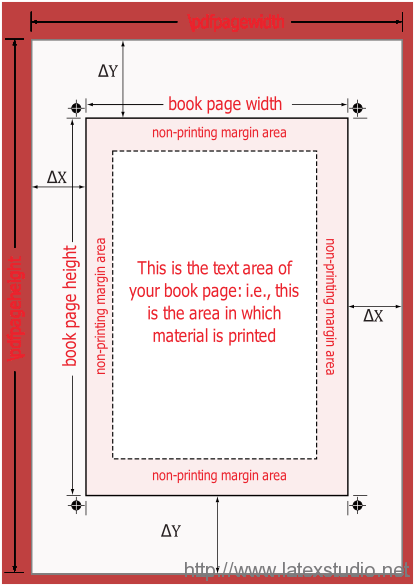
\includegraphics[width=0.8\textwidth, height=8cm]{figures/pagedesign.png}
	\caption{排版}
\end{figure}


%%%%%%%%%%%%%%%%%%%%%%%%%%%%%%%%%%%%%%%%%%%%%%%%%%%%%%%%%%%
%%%%%%%%%%%%%%%%%%%%%%%%%%%%%%%%%%%%%%%%%%%%%%%%%%%%%%%%%%%

\section{章节的类型}

%The basic sections in a book are chapter, section, subsections and so on. 
%These sections will appear in the \imp{tableofcontents} of the book.
基本的章节结构,比如说,第一章,1小节,1.1小节...。对应chapter, section, subsection...。
这些都会出现在目录中,即在正文begin\{document\}之后的tableofcontents中。

你也可以把每一章放在同一个目录下的文件夹中,比如content下面,有这几章ch\_basic.tex, ch\_math.tex, ch\_table.tex。
然后再用\imp{input}, 把他们加载在正文中。这样对于大型的文档,比如书,或者几个人合作写书,特别有好处。
每个人只要写自己的那个部分,最后放在一个文件里面就好了。

比如在这里加载content目录下的ch\_basic.tex篇章,可以用\textbf{\textbackslash input\{content/ch\_basic\}}

%%%%%%%%%%%%%%%%%%%%%%%%%%%%%%%%%%%%%%%%%%%%%%%%%%%%%%%%%%%

\subsection{小节的例子}

This is just one example for a subsection.

%%%%%%%%%%%%%%%%%%%%%%%%%%%%%%%%%%%%%%%%%%%%%%%%%%%%%%%%%%%
%%%%%%%%%%%%%%%%%%%%%%%%%%%%%%%%%%%%%%%%%%%%%%%%%%%%%%%%%%%

\section{基本的页面设置}

为了展示页面的设置,我们用一些电脑随机生成的文字来填充章节,这需要用到\imp{blindtext}这个包。

\blindtext[6]

\blindtext

\blindtext[7]

%%%%%%%%%%%%%%%%%%%%%%%%%%%%%%%%%%%%%%%%%%%%%%%%%%%%%%%%%%%
%%%%%%%%%%%%%%%%%%%%%%%%%%%%%%%%%%%%%%%%%%%%%%%%%%%%%%%%%%%

\section{页眉和页脚}

%The head and foot of the document can be adapted using the packages \imp{fancyhdr}. The using the commands, e.g., \imp{pagestyle\{fancy\}}, \imp{l/c/rhead/foot} or with \imp{fancyhead/foot[EL,CO]} the respective parts can be edited as needed.

修改页眉和页脚可以用包: \imp{fancyhdr}. 使用的命令如:\imp{pagestyle\{fancy\}}, \imp{l/c/rhead/foot} 或者 \imp{fancyhead/foot[EL,CO]},
对应的页眉页脚就会被修改。

%%%%%%%%%%%%%%%%%%%%%%%%%%%%%%%%%%%%%%%%%%%%%%%%%%%%%%%%%%%
%%%%%%%%%%%%%%%%%%%%%%%%%%%%%%%%%%%%%%%%%%%%%%%%%%%%%%%%%%%

\section{New commands and input}

如果命令比较长,或者需要整合一些命令来完成一系列操作,那么重新定义一些新的命令来完成就变的非常有用。在开始导言区, 
使用\imp{newcommand}来定义新的命令。随着时间的增加,你个人使用的命令也越来越多。把这些命令保存到一个文件里面,
要使用的时候就把它拷贝到你的项目目录,然后使用\imp{input}来加载它。

%%%%%%%%%%%%%%%%%%%%%%%%%%%%%%%%%%%%%%%%%%%%%%%%%%%%%%%%%%%
%%%%%%%%%%%%%%%%%%%%%%%%%%%%%%%%%%%%%%%%%%%%%%%%%%%%%%%%%%%

\section{语言}

文档的默认使用语言是英语,我们可以使用包来改变它。比如中文就使用\imp{ctex}, 德文就使用\imp{ngerman}。
基本上都有相应的包支持你的语言。
使用这个包可以把章、图片,表格等等自动转化成中文显示。
但是需要注意的是,写法是\textbf{\\usepackage[UTF8, heading=true]\{ctex\}}。
UTF8是代码的格式,中文一般就使用这个,heading=true,可以使得Chapter变成中文的章字。

%%%%%%%%%%%%%%%%%%%%%%%%%%%%%%%%%%%%%%%%%%%%%%%%%%%%%%%%%%%
%%%%%%%%%%%%%%%%%%%%%%%%%%%%%%%%%%%%%%%%%%%%%%%%%%%%%%%%%%%
%%%%%%%%%%%%%%%%%%%%%%%%%%%%%%%%%%%%%%%%%%%%%%%%%%%%%%%%%%%
